\begin{figure}[h]
	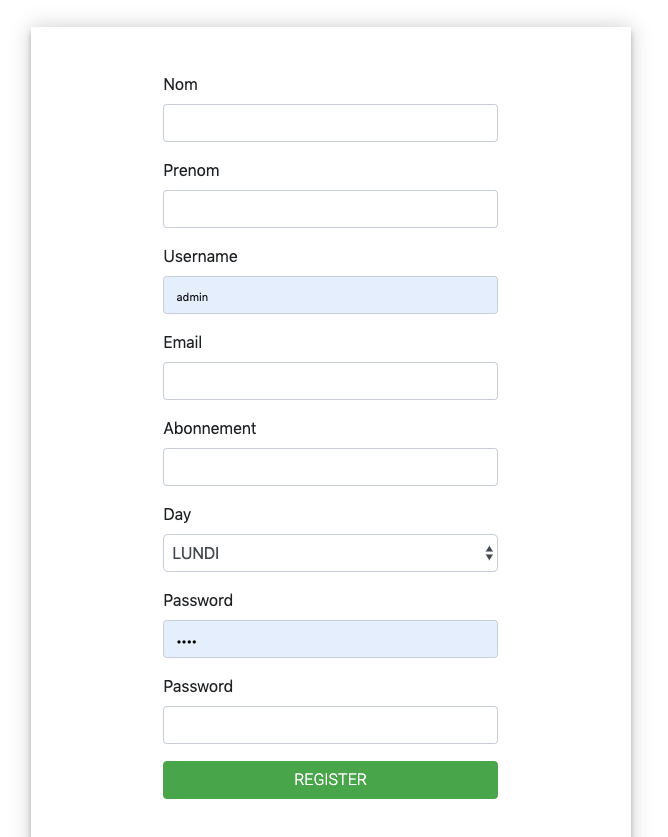
\includegraphics[width=0.5\textwidth,center]{Figures/us1-1}
	\caption{Formulaire d'inscription}
\end{figure}

\vspace{\baselineskip}
\begin{enumerate}
	\item L'utilisateur rentre ses information dans le formulaire. 
	\item L'utilisateur sélectionne le type de session à laquelle il est inscrit. 
	\item L'utilisateur clique sur \textit{Register} et attend la redirection. 
\end{enumerate}

\newpage
\subsubsection{Gestion des erreurs et sécurité}
	\paragraph{}
		\begin{itemize}
			\item L'utilisateur doit remplir tous les champs. Si un champ est manquant, une erreur apparaitra. 
			\item Le nom d'utilisateur et l'adresse Email sont uniques dans le système, s'il entre un Email ou nom d'utilisateur déjà existant, une erreur lui dira de corriger.
			\item L'utilisateur doit confirmer son mot de passe, si les mots de passe sont différents ou plus petits que 6 charactères il y aura un message d'erreur.
		\end{itemize}
		
\subsubsection{Diagramme de séquence}
	\begin{figure}[h]
		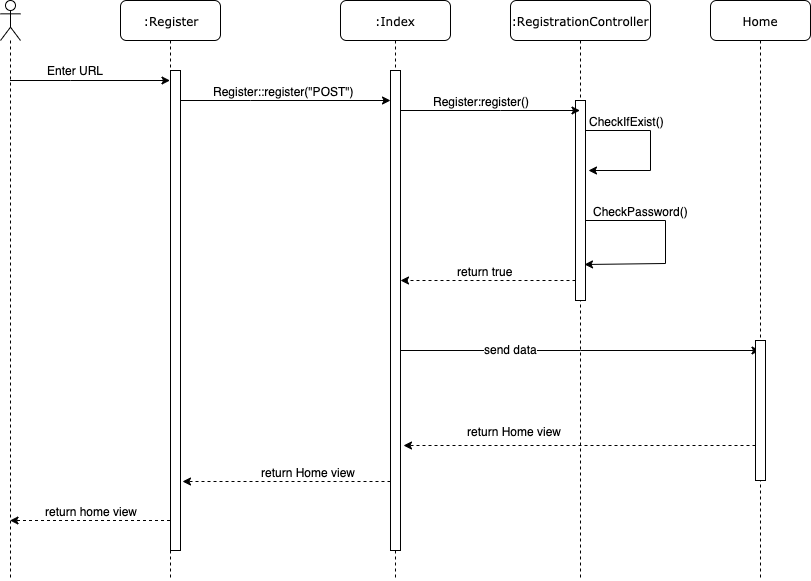
\includegraphics[width=0.8\textwidth,center]{Diagramme/sequence-us1}
		\caption{Diagramme de séquence de l'enregistrement d'un nouvelle utilisateur. }
	\end{figure}
	
	
\subsubsection{Scripts concernés}
	\begin{itemize}
		\item \Href{https://github.com/victorsmits/Aquabike/blob/master/backend/src/Controller/RegistrationController.php}{RegistrationController.php}
		\item \Href{https://github.com/victorsmits/Aquabike/blob/master/backend/templates/registration/register.html.twig}{register.html.twig}
		\item \Href{https://github.com/victorsmits/Aquabike/blob/master/backend/src/Entity/Person.php}{Person.php}
	\end{itemize}